% PLEASE USE THIS FILE AS A TEMPLATE
% Check file iosart2c.tex for more examples
%
% Journal:
%   Journal of Ambient Intelligence and Smart Environments (jaise)
%   Web Intelligence and Agent Systems: An International Journal (wias)
%   Semantic Web: Interoperability, Usability, Applicability (SW)
% IOS Press
% Latex 2e

% options: jaise|wias|sw
% add. options: [seceqn,secfloat,secthm,crcready,onecolumn]


%\documentclass{iosart2c}

\documentclass[sw]{iosart2c}
%\documentclass[wias]{iosart2c}
%\documentclass[jaise]{iosart2c}

\usepackage[T1]{fontenc}
\usepackage{times}%
\usepackage{natbib}% for bibliography sorting/compressing
%\usepackage{amsmath}
%\usepackage{endnotes}
% \usepackage{graphics}
\usepackage{graphicx}

\usepackage{color}
\usepackage{url}
\usepackage{xspace}

%%%%%%%%%%% Put your definitions here

\newcommand{\myurl}[1]{\footnote{\url{#1}}}
\newcommand{\todo}[1]{\textbf{{\color{blue}$\Longrightarrow$ #1}}}

\newcommand{\via}{\emph{via}\xspace}
\newcommand{\perse}{\emph{per se}\xspace}
\newcommand{\ie}{\emph{i.e.}\xspace}
\newcommand{\eg}{\emph{e.g.}\xspace}
\newcommand{\etc}{\emph{etc.}}
\newcommand{\protege}{Prot\'eg\'e\xspace}
\newcommand{\con}[1]{\texttt{#1}\xspace}


%%%%%%%%%%% End of definitions

\pubyear{0000}
\volume{0}
\firstpage{1}
\lastpage{1}

\begin{document}

\begin{frontmatter}

%\pretitle{}
\title{Bringing phytopathology onto the reasoned Semantic Web: the Plant-Pathogen Interactions Ontology (PPIO)}
\runningtitle{}
%\subtitle{}

%\review{}{}{}


% For one author:
%\author{\fnms{} \snm{}\thanks{}}
%\address{}
%\runningauthor{}

%Two or more authors:
\author[A]{\fnms{Alejandro} \snm{Rodr\'iguez Iglesias}\thanks{Corresponding author. Email:alejandroriglesias@gmail.com}},
\author[A]{\fnms{Mikel} \snm{Ega\~na Aranguren}},
\author[A]{\fnms{Alejandro} \snm{Rodr\'iguez Gonz\'alez}} and
\author[A]{\fnms{Mark D.} \snm{Wilkinson}}
\runningauthor{}
\address[A]{Biological Informatics Group, Centre for Plant Biotechnology and Genomics (CBGP), Technical University of Madrid (UPM), Spain}
%\address[B]{}

\begin{abstract}
Interactions between plants and plant-pathogenic bacteria have both scientific and economic importance, and are particularly relevant in the domain of biodiversity. While semantically-oriented resources exist that describe certain aspects of plant phenotypes, biodiversity, and plant disease, few are designed specifically to be used together with rich semantic reasoning, and none are specifically aimed at describing the interplay between plants and the organisms that infect them.  We present here the Plant-Pathogen Interactions Ontology (PPIO), whose axiomatic models allow the integration of, and inference over, plant-pathogen interaction datasets in a semi- or fully-automated manner.
\end{abstract}

\begin{keyword}
 plant pathogenic bacteria \sep ontologies \sep Semantic Web \sep PPIO \sep plant pathology \sep reasoning
\end{keyword}

\end{frontmatter}

%%%%%%%%%%% The article body starts:

\section{Introduction}\label{s1}


Plants can be susceptible to attack by a wide range of pathogenic bacterial genera \cite{Bull2010}. If the plant's defense barriers are overcome, the infection process(es) can ultimately result in the death of the plant. Even if the plant survives, pathogenic processes may have significant effects on economically important traits such as crop yield, and as a consequence there is significant interest in capturing and curating plant/pathogen interaction data \cite{Montesinos}. Unfortunately, plant-pathogen interaction data is largely collected in a highly distributed manner, by many research teams worldwide, and sometimes even by individual land-workers themselves.  As a result, there is a large amount of both structured and unstructured, curated and non-curated, data in this domain of interest, as exemplified by the hundreds of publications that focus their interest on unveiling the mechanisms  by which the pathogenic bacteria interact with their hosts \cite{DeWit,Dodds}. Therefore, construction and integration of unified data sources related to plant interactions with pathogenic bacteria is an essential development. % and will ultimately lead to a better preservation of worldwide crops.

The field of plant-pathogenic bacteria also provides a stark example of the increasing relevance of biodiversity research in the area of plant pathology \cite{Mansfield}. Traditionally, {\itshape Agrobacterium, Erwinia, Pseudomonas and Xanthomonas} were considered the four primary plant pathogenic genera. With the rapid improvement of experimental techniques, the number of identified plant-pathogenic bacteria genera has increased to at least 30. As a result, large amounts of unconnected biological data have been created, and these are archived over a wide range of both structured and unstructured resources. It is, clearly, highly desirable to pursue initiatives that will make these data easier to integrate, explore, and interpret.

The effectiveness of Semantic Web technologies to manage large, distributed datasets has been demonstrated in other areas of the life sciences (See Section \ref{sec:discussion}). However, to date, Semantic Web tools have not been extensively applied to the knowledge domain of plant-pathogenic bacteria. Here we present the Plant Pathogen Interactions Ontology (PPIO), an ontology developed to integrate and organize data about interactions between plants and their (currently bacterial) pathogens. The main goal of PPIO is to serve as a reference for expert plant pathologists by providing the knowledge necessary to assist in their interpretation of, and prediction of, the phenotypic responses that result from pathogenic biological interactions.


\section{Modelling}

The initial data upon which the PPIO was modelled was collected manually by consulting and ``scraping'' a number of different Web resources. The main resource\myurl{http://pseudomonas-syringae.org/} contained diverse state-of-the-art datasets related to various {\itshape Pseudomonas syringae} pathogenic strains. This page also provided a bridge to other Web resources where additional datasets were collected\myurl{http://ncppb.fera.defra.gov.uk/}. After the initial dataset was gathered, filtered, and revised, modelling of the data, and the knowledge within it, was performed using the ontology editor Prot\'eg\'e v4.2.0\myurl{http://protege.stanford.edu}.

\subsection{Design principles and high-level overview of classes}

The main goal pursued during the modelling and designing process was to semantically capture as much of the biological knowledge within the data as possible (Figure \ref{fig:ppio-classes}). In particular, a special effort was made to model the {\itshape disease triangle}\myurl{http://www.apsnet.org/edcenter/instcomm/TeachingArticles/Pages/DiseaseTriangle.aspx}. This idea, one of the cornerstones of plant pathology, asserts that three factors must be present for a disease to occur: a virulent pathogen, a susceptible host, and a propitious environment. Two semantic classes were created to represent these three elements in sufficient richness and precision, namely, the {\sf Environmental parameter} and the {\sf Organism} classes. The later class, intended to model organism taxonomies, is broken into two subclasses that semantically describe either the plant taxonomy, or the pathogenic bacteria's taxonomy. These subclasses are linked to the {\sf NCBITaxon\_1} class, that incorporates both a bacterial and plant genera hierarchy with their corresponding taxon identification number as provided by the National Center for Biotechnology Information (NCBI). Also, terms such as {\sf Plant Pathogen}, {\sf Host Plant} or {\sf Resistant plant} have been strongly axiomatically modelled to deeply capture details within the extracted biological data.  Thereafter, by making use of automated reasoning, members of the {\sf Host Plant} and {\sf Resistant Plant} subclasses can be automatically inferred (Tested using FaCT++ \cite{TsHo06a} and HermiT 1.3.8 \cite{hermit}). As such, the {\itshape reason} that a plant is considered a host, or a bacteria is considered a pathogen, can be determined by exploration of the data, rather than by assertion of this role.

The physiological state of a plant can often be inferred visually by observing its expressed phenotype. Thus, significant effort was also made towards modelling plant phenotypes in the PPIO, in the form of several classes specifically created to meticulously represent plant phenotypic traits. Of particular importance are the {\sf Phenotype} and the {\sf Phenotypic process} classes. These two classes semantically capture the output of the interaction between the host and the bacteria, which is ultimately represented as a resistance or a susceptibility phenotype.

Finally, the {\sf Trait} class contains various physiological, biochemical and molecular plant traits. This class was built by importing the Plant Trait Ontology
% \myurl{http://www.gramene.org} 
\cite{PTO} into PPIO. The traits defined by different PTO classes are used to describe the effects of a bacterial attack on a susceptible host. This is accomplished by axiomatically relating the {\sf Trait} class with both {\sf Phenotype} and {\sf Phenotypic process} classes within the PPIO.


\begin{figure}
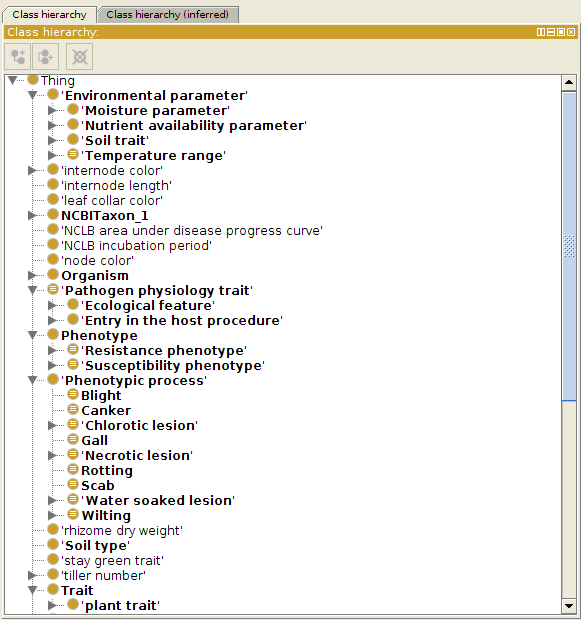
\includegraphics[width=0.5\textwidth]{PPIO-classes2.png}
\caption{General view of the PPIO main classes and subclasses. Classes in bold refer to those newly created for building PPIO; the rest of classes belong to the Plant Trait Ontology.}\label{fig:ppio-classes}
\end{figure}


\section{Creation methodology}

\subsection{URI design}
The ontology URI (\url{http://purl.oclc.org/PPIO}) is HTTP resolvable and permanent (the PURL server redirects to our laboratory's server at \url{biordf.org}, but could redirect to another location if the ontology is ever migrated to a new location). The identifiers for entities (classes, individuals and object properties) are alphanumeric, with a URI of the type \url{http://purl.oclc.org/PPIO#PPIO_NNNNNNN}. Every entity has an informative {\sf rdfs:label} annotation. 

\subsection{Ontology production}
The development of PPIO is automated as much as possible, since it is designed to be expanded to adapt to new species/phenotypes as they are described. The core ontological structure is manually constructed. Subsequently, most of the remaining ontological concepts are produced programmatically using the Galaxy platform, a bioinformatics-oriented workflow environment \cite{galaxy}. Within Galaxy, the workflow required to automatically enrich the PPIO is defined once, and then executed for each release. This also allows us to plug PPIO synthesis directly into other Bioinformatics tools, thus enabling and simplifying additional ontological enrichment in the future.

The workflow adds the necessary entities and axioms\footnote{The workflow and necessary datasets and scripts can be found at the following Galaxy page: \url{http://biordf.org:8983/u/alejandroriglesias/p/ppio-production}} as follows (Figure \ref{fig:galaxy-workflow}):
\begin{enumerate}

\item The organism taxa hierarchy is produced by the tool NCBITaxonomy2OWL\myurl{http://github.com/mikel-egana-aranguren/NCBITaxonomy2OWL}. It retrieves user-defined taxa from the NCBI taxonomy through a BioPortal Web Service \cite{bioportal} and injects these into the PPIO, reproducing the original taxonomical hierarchy (representing each rank-subrank as a simple subsumption relation \cite{taxa_ismb_2008}) and adding each taxon with a resolvable OntoBee\myurl{http://www.ontobee.org/} URI.

\item Since pathogens in PPIO are modelled as OWL individuals, rather than OWL classes, they cannot be directly related with class hierarchies like the NCBI taxonomy and the symptoms hierarchy. Therefore, PPIO exploits OWL punning\myurl{http://www.w3.org/TR/owl2-new-features/Punning}, where an individual with the same URI as each type-class is generated programmatically for those hierarchies. This is achieved by defining two Ontology Pre Processor Language (OPPL)\myurl{http://oppl.sf.net} scripts and executing them via OPPL-Galaxy \cite{OPPL-Galaxy-JBMS} as follows:

{\small 
\begin{verbatim}
?x:CLASS,
?y:INDIVIDUAL = create(?x.RENDERING)
SELECT ?x SubClassOf NCBITaxon_1
WHERE ?x != Nothing, ?x != Thing
BEGIN
ADD ?y Type ?x
END;
\end{verbatim}
}

{\small 
\begin{verbatim}
?x:CLASS,
?y:INDIVIDUAL = create(?x.RENDERING)
SELECT ?x SubClassOf PPIO_0000069
WHERE ?x != Nothing, ?x != Thing
BEGIN
ADD ?y Type ?x
END;
\end{verbatim}
}

\end{enumerate}

The linking of pathogens to those hierarchies (\eg, using Manchester OWL Syntax, {\sf NCBITaxon\_552 Types Erwinia amylovora}, {\sf NCBITaxon\_552 causes symptom Canker}, {\sf NCBITaxon\_552 causes symptom Blight}) is done later manually. Through our use of OPPL, any complex axiomisation - not only punning - can be defined once and automatically applied every time the workflow is executed, complying with current best practices for scientific computing, since we automate as much as possible the manipulation of PPIO \cite{bp_computing}.

\begin{figure}
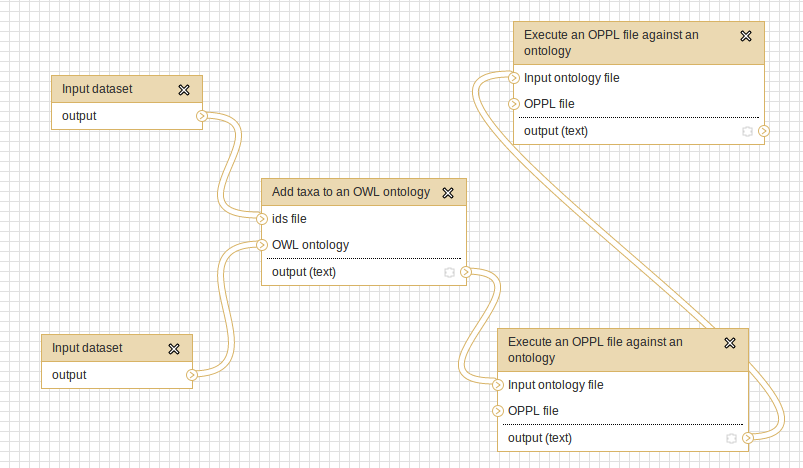
\includegraphics[width=0.5\textwidth]{galaxy-workflow.png}
%{galaxy-workflow}
\caption{Galaxy workflow for producing a release of PPIO. In the first step, NCBITaxonomy2OWL is executed; it gets the ontology and a flat file containing the NCBI taxonomy IDs, and it adds them to the ontology. Then two OPPL scripts are executed against the resulting ontology, adding axioms and entities to create and individual for each class in the hierarchies under {\sf NCBITaxon\_1} and {\sf PPIO\_0000069}.}\label{fig:galaxy-workflow}
\end{figure}


\section{Discussion}\label{sec:discussion}


Semantic-oriented initiatives like the OBO foundry \cite{Smith}, which includes Gene Ontology \cite{Gene}, Bio2RDF \cite{RDF} or the W3C Semantic Web for Health Care and Life Sciences Interest Group\myurl{http://www.w3.org/blog/hcls/} have provided copious evidence supporting the successful application of semantics to the problem of automated data integration and exploration. Nevertheless, within the fields of plant biotechnology and phytopathology, it is surprising how limited the application of these powerful technologies have been, and to how few resources. Some notable exceptions include the Plant Ontology\myurl{tp://www.plantontology.org/}, which describes plant anatomy, morphology and developmental stages \cite{PO}; and the Plant Disease Ontology (IDOPlant) \cite{Walls} \cite{IDO}, which is focused on generically describing plant infectious diseases. Comparison between the IDOPlant and PPIO will reveal that the former constructs a more general model of infection where, for example, plant infectious diseases are described as being caused by either biotic or abiotic agents. The PPIO ontology, in contrast, pursues a knowledge capture strategy focused on more detailed data concerning interactions between plants and their pathogens, and the consequences of those interactions. Finally, the GO extension for description of the Type III Effectors \cite{Lindeberg} is the contribution in the plant pathology and microbiology area most related to PPIO. With this in-mind, the GO extension for type III effectors is designed to capture information about processes at the host-pathogen level, but with a strong emphasis on effector protein data. PPIO acts as a more generalized knowledge base; as such, the PPIO fills a gap in description of pathogenic interactions that does not significantly overlap with (and in fact, explicitly utilizes and extends) other relevant semantic resources.  Our objective in the future is to continue integrating data and other knowledge resources, such as Darwin Core (DwC) \cite{Wieczorek2013}. The end-goal is to create a platform that, combined with others, could act as a key component within a diagnosis/prevention/alert system, much like clinical decision support systems in the medical domain. For example, PPIO will make it possible for users to pose, and answer, questions such as:

\begin{enumerate}
\item Is {\itshape Solanum lycopersicum} susceptible to {\itshape Pseudomonas syringae} pv. {\itshape tomato} DC3000?
\item Does a high humidity favours the development of {\itshape Pectobacterium carotovorum} subsp. {\itshape carotovorum}?
\item What is the phenotype of the disease produced by {\itshape Dickeya dadantii} in {\itshape Solanum tuberosum}?
\item What is the host range of the pathogen {\itshape Pseudomonas marginalis} pv. {\itshape marginalis}?

\end{enumerate}

Knowledge acquisition is the process of converting knowledge from unstructured sources into a format that is more rigorously processable. As datasets become larger, and as expert knowledge continues to be broadly dispersed, it becomes increasingly necessary to automate the capture of relevant knowledge, and optimally, to automate the addition of this knowledge into a rich ontological context. However, while the PPIO represents a framework for capturing rich plant/pathogen interaction data in a machine-processable manner, we continue to rely on field experts to ensure the accuracy of the data content captured within it. To this end, we are pursuing a knowledge capture project specifically aimed at accurately collecting relevant, manually-verified data {\itshape en masse}, that will ultimately populate the PPIO knowledge base. A preliminary prototype is available\myurl{http://1.tfguc3m.appspot.com/}. By logging in, users can choose among different and suitable expert profiles. Afterwards, a series of questions will be available, depending on the profiles selected. Once the percentage of the given answers have been evaluated and curated by different approaches, the datasets will be ready for the step of populating the PPIO. We hope, thereby, to achieve the objective of making PPIO an essential bioinformatics tool for the plant-pathogen community.

% Knowledge acquisition is the process of converting knowledge from unstructured sources into a format that is more rigorously processable. 


\section*{Acknowledgements}
Alejandro Rodr\'iguez Iglesias, Alejandro Rodr\'iguez Gonz\'alez and Mark D Wilkinson are funded by the Isaac Peral Programme. Mikel Ega\~na Aranguren is funded by the Marie Curie-COFUND Programme (FP7) of the EU.




%\begin{figure}[t]
%\includegraphics{}
%\caption{Figure caption.}\label{f1}
%\end{figure}

%\begin{table*}
%\caption{} \label{t1}
%\begin{tabular}{lll}
%\hline
%&&\\
%&&\\
%\hline
%\end{tabular}
%\end{table*}


%%%%%%%%%%% The bibliography starts:
%\begin{thebibliography}{9}

%\bibitem{r1}

%\bibitem{r2}

%\end{thebibliography}

\bibliographystyle{abbrv}
  \bibliography{swj_ppio}

\end{document}
